\documentclass[10pt,twocolumn,letterpaper]{article}
\usepackage[pagenumbers]{cvpr}
\usepackage[UTF8,scheme=plain,fontset=fandol]{ctex}
\usepackage{mathtools,tabularx,multirow,balance}
\usepackage{tikz}
\usetikzlibrary{arrows.meta,positioning,fit,backgrounds}
\usepackage[breaklinks,colorlinks,citecolor=blue,urlcolor=blue,linkcolor=blue]{hyperref}
\renewcommand{\abstractname}{摘要}
\patchcmd{\abstract}{Abstract}{摘要}{}{\errmessage{Cannot localize abstract}}
\renewcommand{\refname}{参考文献}
\renewcommand{\figurename}{图}
\renewcommand{\tablename}{表}
\newcommand{\R}{\mathbb{R}}
\newcommand{\code}[1]{\texttt{\small #1}}
\def\confName{CVPR}
\def\confYear{2026}
\title{基于动态人—物交互图与选择性状态空间模型的\\行为意图预测：系统实现与小规模实验}
\author{项目技术报告\\2026 年 11 月 12 日 · 本地证据核验版}
\begin{document}
\maketitle

\begin{abstract}
行为意图提前预测需要从连续观测中同时判断参与交互的主体、目标对象与关系变化。面向这一问题，本文整理一套从第一视角视频、双手姿态与二维实例观测到未来有向交互图的实现方案。系统使用统一实体编码器表达左手、右手、双手组合和物体，以帧内注意力融合空间上下文，再通过共享 Mamba 时序骨干与有向实体对预测头，输出至少一秒之后的多标签关系。针对标注稀疏与遮挡，系统分离明确正例、明确负例和未知状态，仅对有证据的单元计算损失；针对潜在未来信息泄漏，窗口选择和模型输入限定在历史观测内。现有冻结资源池包含 300 段采集、868,255 个原生帧，其中已准入的交互训练子集为 5 段采集、1,238 个窗口。已有训练记录显示，Mamba、LSTM 与因果 Transformer 均完成 50 轮训练，测试 micro-F1 分别为 0.4761、0.4801 与 0.5609。本文进一步根据标签计数复算全正预测参照值 0.5354，说明当前证据尚不足以支持 Mamba 的性能优势。报告给出数据协议、模型实现、实验解读以及 demo 素材方案，形成可继续补充原始运行记录和扩大评估规模的技术基线。
\end{abstract}

\section{引言}
在人机协作、机电装配和辅助操作中，感知系统不仅要识别已经发生的动作，还需要在动作执行前判断操作者接下来可能与哪个对象发生何种交互。例如，双手接近桌面既可能是拾取工具，也可能是稳定工件；手部与物体保持接近也不一定意味着已建立抓持。单一视频类别难以完整表达这种主体、客体和交互状态之间的结构关系。

本项目将行为意图具体化为\textbf{未来交互关系的预测}。该操作性定义不直接测量人的心理状态，而是在历史视觉观测给定时，预测未来时刻的接触、抓持、操作与协作等可观察变量。目标表示采用有向多标签图：节点对应手或物体，边对应主体作用于客体的关系，同一实体对可以同时具有多个标签。例如，右手可以同时与某个物体接触并控制其运动，工具还可以作用于第二个工件。

这一问题的主要困难来自三个方面。首先，物体身份和姿态受遮挡、形变与相机运动影响，二维可见范围、局部表面位姿和整物体六自由度位姿不能混为一谈。其次，稀疏标注中未被检查的关系不是负例；错误填充会使学习目标偏向大量伪负样本。最后，离线标注常利用后续帧建立稳定身份或几何，如果这些结果进入历史输入，预测模型就可能利用未来信息。

本文的工程贡献包括：一套保留原生时基与来源记录的数据处理和训练准入机制；一套面向部分可见实体的帧内关系编码、共享时间建模与有向图解码实现；以及同输入、同监督下的三骨干训练对照和逐项证据分析。现有工作是\textbf{条件化交互预测系统与小规模实验}，开放场景泛化、完整物体姿态预测和长期在线运行仍需独立验证。

\paragraph{资料范围。}
本文的代码、数据索引和审计计数来自本地冻结文件，训练指标来自 2026 年 10 月 24 日训练报告。编写时未能连接远端服务器，故未重新读取三组训练的 checkpoint、逐轮日志和 benchmark JSON。表格明确区分文档转录值与本次计数推导值；若服务器已有后续实验，应按附录列出的文件更新结果，而不能将本稿视为远端最新状态的确认。

\begin{figure*}[t]
\centering
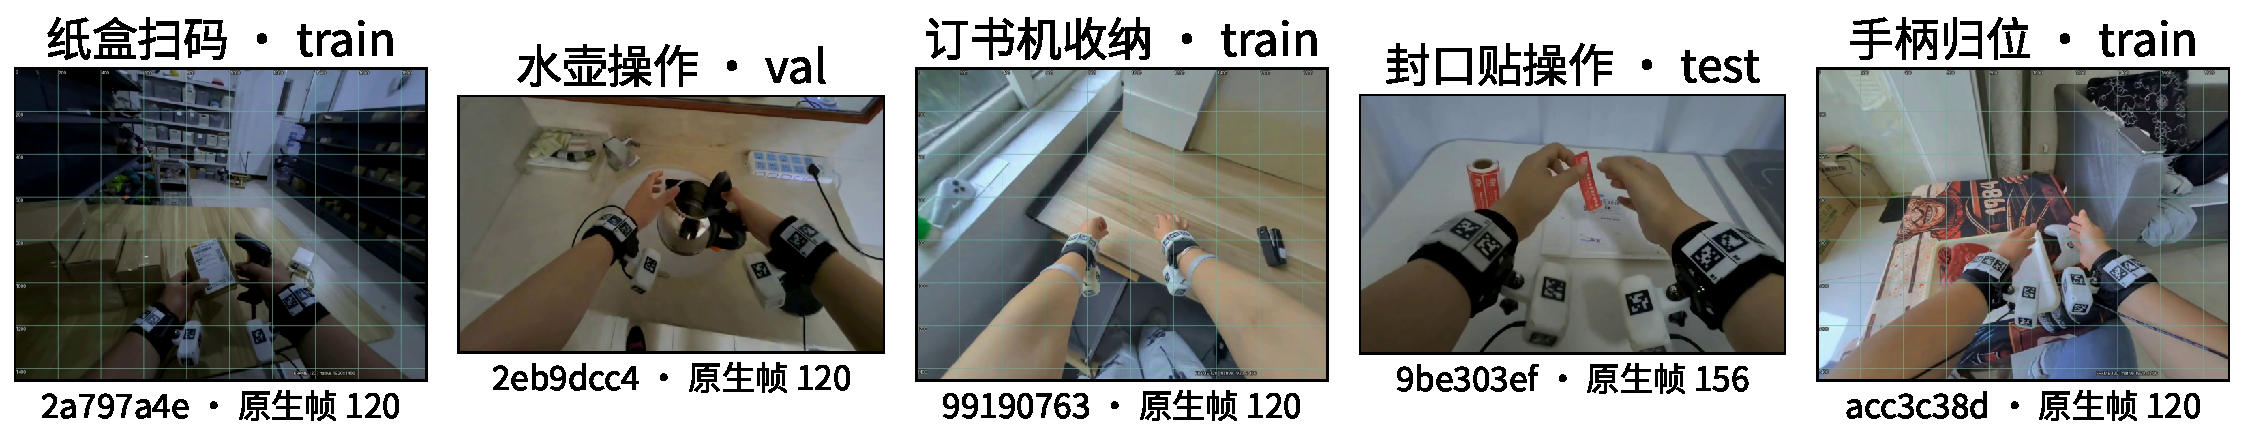
\includegraphics[width=\textwidth]{figures/dataset_examples.pdf}
\caption{已准入 V5 子集的五段采集。使用已保存的标注版左目证据帧：测试为第 156 帧，其余为第 120 帧；训练场景图保留原审核坐标网格。训练为纸盒扫码、订书机收纳和手柄归位，验证为水壶操作，测试为封口贴操作。这里展示场景内容，不表示该帧具有完整标签或模型预测正确。证据图来源、图像 SHA-256 与视频 LFS 对象标识保存在配套清单中。}
\label{fig:data}
\end{figure*}

\section{相关工作与技术定位}
\paragraph{第一视角活动理解。}
EPIC-KITCHENS-100 将第一视角活动研究扩展到动作识别、检测和提前预测等任务\cite{damen2022rescaling}；Ego4D 则提供覆盖多种日常活动的大规模第一视角视频资源\cite{grauman2022ego4d}。这些工作说明连续活动和未来行为具有实际研究价值。本文不在其公开测试集上报告成绩，也不把不同数据集、标签粒度和输入条件下的数字放入同一性能排名。当前实验使用 EgoDemo 的本地冻结子集\cite{egodemo}，研究对象是有明确实体引用的未来交互图。

\paragraph{手部与物体感知。}
MediaPipe Hands 通过手掌检测和关键点网络实现图像中的手部跟踪\cite{zhang2020mediapipe}。FoundationPose 提供面向新物体的六自由度位姿估计和跟踪框架，支持 CAD 模型或参考图像条件\cite{wen2024foundationpose}。本项目的独立感知试验集成了这两类方法；但 V5 训练的手部输入来自数据集官方姿态，物体输入使用经审核的二维观测。将独立感知演示直接称为 V5 全自动端到端推理，会掩盖这一输入差异。

\paragraph{时间建模。}
Mamba 通过输入依赖的选择机制控制状态更新，并在序列长度方向具有线性扩展特性\cite{gu2023mamba}。本文复用其时间骨干，配合项目自建的实体编码器与图预测头；并不声称提出新的状态空间算子。LSTM 与因果 Transformer 用于检验同一关系表示下不同时间骨干的行为。由于当前窗口仅有 32 帧，长序列优势尚不能由现有实验推出；时延和显存优势也需要同硬件、同批量、同精度的测量。

\section{问题定义与数据协议}
\subsection{预测对象与因果时间窗}
令历史截止帧为 $t$，原生时间戳为 $\tau_t$，窗口长度为 $W=32$。实体集合最多含 $E=11$ 个节点：左手、右手、双手组合以及至多八个物体。模型输入为
\begin{equation}
 X_t\in\R^{W\times E\times120},\quad
 V_t\in\{0,1\}^{W\times E},
\end{equation}
其中 $V_t$ 指示每帧实体观测是否有效。目标帧 $u$ 满足
\begin{equation}
 \tau_u-\tau_t\geq 1\ \mathrm{s}.
\end{equation}
实际间隔依照原生时间戳计算，不以固定 30 帧替代一秒，也不插值生成目标。窗口从历史起点到未来目标应处在连续复核范围内，以保证目标状态有可追溯依据。

预测为 $\hat P_t\in[0,1]^{E\times E\times K}$，$K=66$ 为冻结词表容量。每个元素对应源实体、目标实体与交互类型。操作、关系和协作标签描述目标帧的已知状态；转换标签描述在预测区间内完整落入的、已确认发生的事件范围。两种时间语义分开解释：转换事件的概率不能解码成精确接触时刻。

\subsection{资源池、训练子集与划分}
冻结资源池含 300 段独立采集、75 个原始任务和 868,255 帧，按采集保持 train/val/test 为 210/45/45。资源池数量描述数据范围，并不等于已完成全部标签的训练样本数。经连续视觉复核、二维实例跟踪质检和窗口审计后，V5 可训练交互子集为五段采集，统计见表~\ref{tab:data}。

\begin{table}[t]
\centering\small
\setlength{\tabcolsep}{4pt}
\begin{tabular}{lrrrr}
\toprule
划分 & 采集 & 窗口 & 正单元 & 负单元\\
\midrule
train & 3 & 592 & 1,953 & 1,452\\
val & 1 & 366 & 1,172 & 406\\
test & 1 & 280 & 786 & 1,364\\
\midrule
合计 & 5 & 1,238 & 3,911 & 3,222\\
\bottomrule
\end{tabular}
\caption{由冻结覆盖报告与独立窗口审计核对的数据统计。监督单元按窗口重复计数；1,238 个重叠窗口不是 1,238 次独立采集。}
\label{tab:data}
\end{table}

V5 共连续复核 1,995 个唯一原生帧，四段已整段查看；扫码采集仅含已查看的连续区间。212 个状态段和有界事件记录用于构造监督。物理转换含 42 个确认发生范围与八个删失范围，另有两个照明变化记录；尚无精确物理转换帧的认证。原始资源池的完整标注状态与整物体 6D 认证仍为未完成，这不阻止在明确范围内使用已准入的交互子集。

实际监督正例类型的并集为 21 类，训练仅有 12 类正例，另九类只在验证或测试中出现。66 是模型输出容量，不是已充分学习的动作类别数。数据按采集隔离，尚未建立充分的跨被试隔离证据，因此本稿不报告跨被试泛化结论。

\subsection{标注来源与未知状态}
交互标签属于助手视觉复核产生的银标，保存证据帧、原生半开区间、主体与客体引用，以及遮挡、删失和无法判断的原因。用户对子集的交付验收不改变逐条标签的来源，不能将银标改称独立人工金标准。

每个图单元保存值 $Y_{ijk}\in\{0,1\}$ 和有效掩码 $M_{ijk}$。只有明确正负记录满足 $M_{ijk}=1$；其余位置即使数值占位为零，也表示未知。跨窗口重复出现的同一状态会产生多个监督单元，因此表~\ref{tab:data} 不能作为独立事件数。按全张量容量计算，明确监督仅为 $7,133/(1,238\times11\times11\times66)\approx0.072\%$；其余容量还包括填充实体和不适用组合，不能把该比例直接解释为实际可行关系的标注覆盖率。

\begin{figure}[t]
\centering
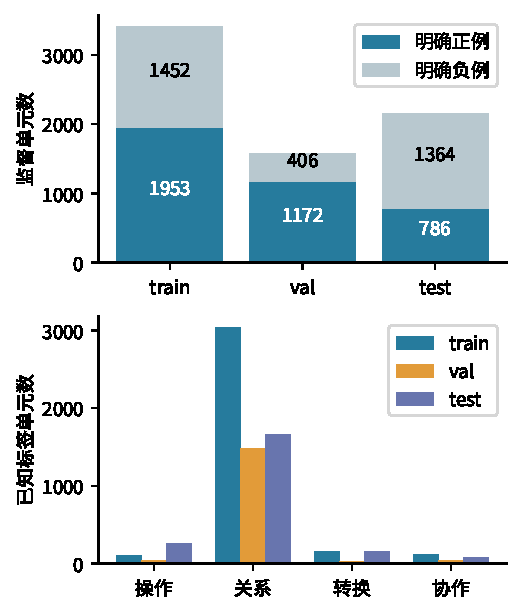
\includegraphics[width=\linewidth]{figures/supervision.pdf}
\caption{监督构成。上：明确正负单元；下：操作、关系、转换与协作四层的已知单元数。关系层占较大比例，聚合 micro-F1 更易受高频关系影响。}
\label{fig:supervision}
\end{figure}

\subsection{实例观测与几何边界}
二维实例输入由当前帧种子启动前向跟踪，最多延续 30 帧，只保留种子存活点，不从未来种子反向补全。历史 32 帧中至少有八帧接受观测的对象才可进入物体槽，按过去首次出现帧和稳定 ID 排序选取至多八个。未来才出现的实体不会预先占据输入槽。

实际质检覆盖 2,667 个候选物体帧，其中 2,357 个接受、310 个拒绝。拒绝原因包含跟随手腕漂移、局部框替代整物体以及严重遮挡。二维框与 RGB 统计提供的是可见观测，而不是精确物体轮廓或完整 6D 真值。离线双向几何估计不进入 V5 编码器；局部部件、非刚体表面和整物体刚体位姿也分别记录。该设计使缺失保持显式，但仍依赖经审核的初始化，尚非纯原始 RGB 的全自动流程。

\section{动态交互图预测方法}
\subsection{统一实体特征}
每个实体使用 120 维向量：归一化二维框四维、历史速度二维、框内 RGB 均值与标准差六维、手部二维关节 42 维、三维关节 63 维，以及有效性和种子标记三维。物体不具备的手关节字段置零，双手组合节点不伪造独立骨架。无效特征在进入可学习层前通过 $V_t$ 清零，避免 NaN 经线性层污染梯度。三维手姿态统一到历史末帧左相机坐标系，长度单位为米。

节点类别编码仅区分左手、右手、双手与物体四种角色。所有物体共享同一类别嵌入，不加入槽位编号嵌入。具体中文名称与稳定 ID 仅用于输出解释，不作为模型特征；未来标签、审核文本和目标元数据同样不进入编码器。

\begin{figure*}[t]
\centering
\resizebox{\textwidth}{!}{%
\begin{tikzpicture}[>=Latex,box/.style={draw=blue!45!black,fill=blue!4,rounded corners=2pt,align=center,minimum height=1.25cm,text width=2.8cm,font=\small},arr/.style={->,thick,draw=blue!60!black}]
\node[box] (input) at (0,0) {历史实体观测\\$32\times11\times120$\\有效掩码 / 节点类别};
\node[box] (space) at (3.65,0) {共享特征投影\\帧内实体注意力\\$32\times11\times128$};
\node[box] (time) at (7.3,0) {逐实体共享时序骨干\\Mamba / LSTM /\\因果 Transformer};
\node[box] (pair) at (10.95,0) {历史末端实体状态\\有向实体对组合\\$[h_i,h_j,h_i-h_j,h_i h_j]$};
\node[box] (output) at (14.6,0) {多标签交互图\\$11\times11\times66$\\逐类型 sigmoid};
\draw[arr] (input)--(space);\draw[arr] (space)--(time);\draw[arr] (time)--(pair);\draw[arr] (pair)--(output);
\node[draw=orange!70!black,fill=orange!7,rounded corners,align=center,text width=8cm,font=\small] (label) at (10.9,-1.65) {未来银标 $Y$ + 已知掩码 $M$：只进入监督与评估\\未知单元不计损失；未见实体不可预测};
\draw[->,dashed,thick,draw=orange!70!black] (output.south)--(label.north east);
\node[align=center,font=\small,text width=6.7cm] at (2.2,-1.6) {输入截止于历史锚点 $t$\\目标帧满足 $\tau_u-\tau_t\geq1$ 秒};
\end{tikzpicture}}
\caption{系统实现。帧内注意力建模空间上下文，时间骨干沿各实体历史独立且共享地运算；末端有向图头保留主体与客体的区别。三骨干对照仅替换时间模块。虚线表示损失与标签的关联，标签不进入前向特征。图为实现结构示意，不是实验输出。}
\label{fig:architecture}
\end{figure*}

\subsection{帧内关系编码}
首先用共享两层感知机将实体特征投影至 $d=128$ 维，再加入实体类别嵌入。每帧的所有有效实体共同参与四头注意力：
\begin{align}
 Z_{s,i}&=\phi(X_{s,i})+e_{\kappa(i)},\\
 \widetilde Z_s&=\operatorname{LN}\big[Z_s+
 \operatorname{Attn}(\operatorname{LN}(Z_s);V_s)\big].
\end{align}
无效实体作为 key 被屏蔽，输出也重新置零。若整帧没有有效观测，实现暂时保留一个零值 key 防止全负无穷 softmax 产生 NaN，再屏蔽该帧所有输出。该步骤处理数值稳定性，不把缺失帧变为有效观测。

帧内注意力让手部节点能依赖附近物体的状态，同时使物体表示包含其他实体的上下文。这里的注意力权重不是物理接触标签，模型最终是否识别接触仍需由独立监督检验。

\subsection{共享时间骨干}
将张量由 $B\times W\times E\times d$ 重排为 $(BE)\times W\times d$，使用共享两层时间骨干建模每个实体的历史。在 Mamba 分支中，状态维数为 16，局部卷积宽度为 4，扩展倍率为 2。选择性状态更新可抽象写作
\begin{align}
 H_{s,i}&=\overline A_{s,i}H_{s-1,i}
             +\overline B_{s,i}\widetilde Z_{s,i},\\
 O_{s,i}&=C_{s,i}H_{s,i},
\end{align}
其中与输入相关的系数选择保留哪些历史信息；实际计算使用现成的 \code{mamba\_ssm} 实现。此式说明机制，并不省略后声称为完整软件层公式。

LSTM 分支采用相同宽度和层数的循环时间模块。Transformer 分支使用可学习时间位置编码、上三角因果屏蔽和四倍宽度的前馈层。三者共享实体编码器、图头、输入、标签与优化规则，但参数量不保证相等，因此本实验是接口和训练协议对齐的骨干比较，不是等参数量或等算力的严格对照。

历史中曾出现但在后续帧缺失的实体允许保留时间状态；从未出现的实体始终屏蔽。固定物体槽并不等于固定物理身份；只有在历史观察提供对应依据时，该节点才具备可解释的实体引用。

\subsection{有向图解码与损失}
在窗口末端提取实体状态 $h_i$，按有序实体对组合
\begin{equation}
 r_{ij}=[h_i;h_j;h_i-h_j;h_i\odot h_j],
\end{equation}
并通过共享感知机产生 $K$ 个 logits $\ell_{ij}$。顺序拼接和差向量保留方向性，使“手作用于物体”和“物体受到手作用”不会被自动视作同一边。每类独立 sigmoid 适用于多标签关系，不使用互斥 softmax。图头支持手到物体以及物体到物体的组合；下游解释仍须遵守类型语义，不能把任意高分组合都认作物理上有效的交互。

令 $Q_{ij}$ 表示源和目标均在历史中出现。训练仅使用既有标注又满足预测条件的单元：
\begin{equation}
 \mathcal L=\frac{1}{|\Omega|}
 \sum_{(i,j,k)\in\Omega}
 \operatorname{BCEWithLogits}(\ell_{ijk},Y_{ijk}),
\end{equation}
其中 $\Omega=\{(i,j,k):M_{ijk}=1,\ Q_{ij}=1\}$。实现会拒绝指向历史未见实体的监督，而不是悄悄丢弃该项。未知单元不进入损失，FP32 累积 BCE 以降低混合精度误差；空监督 batch 必须显式跳过或报告，不能冒充有效训练。

物体槽位置换只改变节点排列；共享类别编码、帧内集合注意力、共享时间模块和共享实体对头使图预测随槽位相应置换。已有冒烟审计记录的最大绝对差为 $1.788\times10^{-7}$。这证明特定检查下的实现一致性，不等于在任意身份错误下仍能正确预测。

\section{实验设置与结果}
\subsection{实现和训练协议}
数据加载绑定冻结索引、数组和审核凭据的 SHA-256，防止修改输入后继续沿用旧的训练许可。默认配置使用 seed 20261024、batch size 16、学习率 $3\times10^{-4}$、权重衰减 0.01、梯度裁剪 1.0，训练 50 epoch，dropout 为零；优化器为 AdamW，启用 BF16 自动混合精度。最优 checkpoint 按验证损失选择，评估阈值为 0.5。

训练记录报告实验运行于 NVIDIA L40 环境。工程验收使用 PyTorch 2.6.0+cu124 和 Mamba 2.2.6.post3。表~\ref{tab:results} 的最终指标来自保存的训练文档，而非本次重新执行模型得到的数值。原始运行目录中的最终配置、最优轮次、参数量、checkpoint 哈希和逐窗口预测尚需远端核验；默认配置不能代替每次运行的实际 manifest。

\subsection{评价指标及统计参照}
只在明确已知标签单元上累积 TP、FP、FN 和 TN，计算
\begin{equation}
 F_1^{\mathrm{micro}}=\frac{2\mathrm{TP}}
 {2\mathrm{TP}+\mathrm{FP}+\mathrm{FN}}.
\end{equation}
macro-F1 对当前 split 中具有已知监督的类型求平均，seen/unseen 则按训练是否出现正例划分。现有实现另提供只对有正例类型取平均的指标，因此不应把这些不同 macro 定义混写。训练没有正例的类型所得分数只反映当前输出与稀疏标签的对应，不能独立证明零样本语义理解。

为量化标签比例的影响，加入不需要训练的全正和全负预测。若已知单元中正例为 $P$、负例为 $N$，全正预测的 micro-F1 为
\begin{equation}
 F_1^{\mathrm{all+}}=\frac{2P}{2P+N}.
\end{equation}
据冻结统计，本次复算得到验证集 0.8524、测试集 0.5354。全负预测在存在正例时 F1 为零。参照线使用相同监督计数，在远端原始评估文件取回后还需核对逐运行的有效单元总数是否一致。

\begin{table*}[t]
\centering\small
\setlength{\tabcolsep}{6pt}
\begin{tabular}{lrrrrrrr}
\toprule
 & \multicolumn{3}{c}{验证集（1 段采集，366 窗口）} & \multicolumn{4}{c}{测试集（1 段采集，280 窗口）}\\
\cmidrule(lr){2-4}\cmidrule(lr){5-8}
模型 & BCE & micro-F1 & macro-seen & BCE & micro-F1 & macro-seen & macro-unseen\\
\midrule
Mamba & 0.6293 & 0.7346 & 0.9151 & 0.6634 & 0.4761 & 0.6519 & 0.4505\\
LSTM & 0.6070 & 0.8027 & 0.9349 & 0.6474 & 0.4801 & 0.6565 & 0.7226\\
Transformer & 0.7064 & 0.6442 & 0.8788 & 0.6540 & 0.5609 & 0.7112 & 0.4708\\
\midrule
全正预测（计数推导） & --- & 0.8524 & --- & --- & 0.5354 & --- & ---\\
全负预测（计数推导） & --- & 0.0000 & --- & --- & 0.0000 & --- & ---\\
\bottomrule
\end{tabular}
\caption{三骨干结果与统计参照。模型数值逐项转录自本地 \texttt{V5\_TRAINING\_20261024.md}，阈值 0.5；全正／全负行由冻结正负单元计数推导，未伪造损失或未计算的 macro 指标。仅包含当前三组运行，没有独立重复训练方差或显著性区间。}
\label{tab:results}
\end{table*}

\begin{figure}[t]
\centering
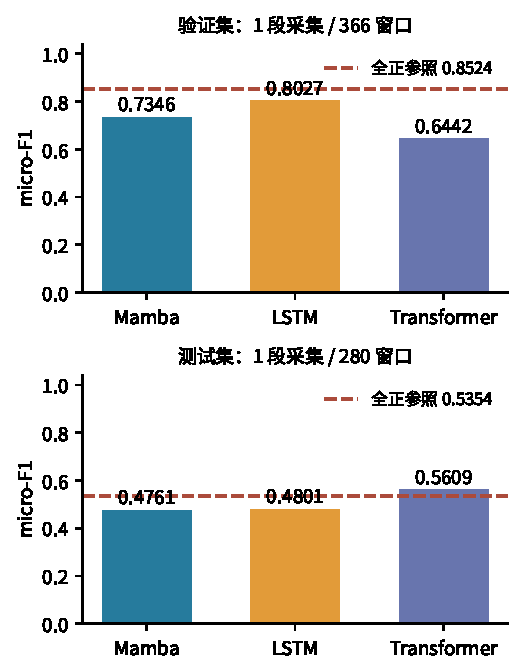
\includegraphics[width=\linewidth]{figures/backbone_results.pdf}
\caption{相同已知监督口径下的 micro-F1 与全正预测参照。柱值来自已有训练报告，虚线由冻结计数复算；没有独立重复运行，故不绘制误差条。}
\label{fig:results}
\end{figure}

\subsection{结果解读}
验证集上，LSTM 的 micro-F1 为 0.8027，高于 Mamba 与 Transformer；但三者均低于全正预测参照。验证集的已知标签正例比例为 $1,172/1,578\approx74.27\%$，仅依靠较多正预测就可能获得较高 F1。因此，验证 F1 较高并不自动意味着模型学到了充分的实体选择与关系判断能力。

测试集上，Transformer 的 micro-F1 最高，为 0.5609，较 Mamba 高 8.48 个百分点，较全正参照仅高约 2.55 个百分点。Mamba 和 LSTM 均低于该参照。已有训练报告给出的 Transformer 测试 precision 为 0.4437，提示应进一步检查假阳性，而不能只依据 F1 排名判断实际可用性。测试集已知正例比例约为 36.56\%，与验证集差异明显，且任务和实体组成同时变化；当前实验不能将性能变化单独归因于某一种分布偏移。

LSTM 的测试 macro-unseen 数值为 0.7226，但该组由少量、并不均衡的已知单元构成，模型也没有为未见类型接收语义描述。应在原始每类计数和预测记录上核查其来源，避免把高分解读成开放词表能力。当前 1,238 个窗口高度重叠，验证与测试又各只有一个采集，逐窗口重采样不能产生可靠的跨采集置信区间。

这些结果说明三种时间骨干已能在一致接口下完成训练和评估；它们没有证明 Mamba 优于基线，也尚未证明学习模型能稳定超越简单统计策略。接下来应优先扩大独立采集和已知负例覆盖，再比较模型结构，而非仅在单段验证序列上反复调整阈值。

\subsection{工程验证与独立感知演示}
V5 的全部 1,238 个窗口已通过独立加载和计数审计。历史输入不受未来标签或元数据改变影响，未知 logit 的直接梯度为零，真实 Mamba 的 FP32/BF16 前后向检查产生有限且非零的梯度。自动复核流水线覆盖 300 段资源，记录零结构错误，同时保留数值告警和待确认问题。上述结果用于评价实现正确性，不作为模型精度或全量标注完成的替代指标。

另一个独立试验在 DexYCB 真人持碗序列上实现了 MediaPipe 手部与 FoundationPose 的同帧输出。44 帧短序列三次复测的稳态生产吞吐为 41.409--41.524 FPS，单帧环路 P95 为 27.056--27.967 ms，每次仍有 2/43 个稳态慢帧。该演示可说明感知模块的集成，但输入是第三人称录制 RGB-D 回放，使用配套首帧 mask 和物体模型；吞吐不是相机到屏幕延迟，也不等于第一视角交互预测端到端速度。44/44 联合输出是覆盖率，独立姿态准确率尚未评估。

\section{定性证据与演示设计}
\subsection{当前可以展示的证据}
图~\ref{fig:timeline} 展示测试采集中的真实连续状态记录。蓝色和橙色分别为已确认正负，灰色保留未判断区域。该图有助于说明：状态可持续、多条关系可以并存、未知不能被平滑地填成负例。它是标注证据图，不是预测性能图。

\begin{figure}[t]
\centering
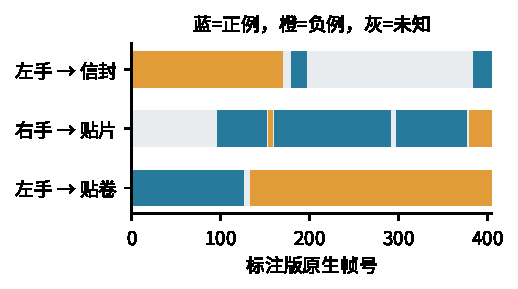
\includegraphics[width=\linewidth]{figures/annotation_timeline.pdf}
\caption{封口贴测试序列的接触状态时间线，直接由冻结复核 JSON 绘制。这里只选择三条关系展示标注机制，未增加人工判断，也未将银标画成模型预测。}
\label{fig:timeline}
\end{figure}

本地实际可用素材包括五个场景的审核证据图、审核页面截图、真人手物同帧感知视频，以及独立的未来姿态探索视频。五段场景的备份 MP4 经文件头检查均为 Git LFS 指针，原视频内容需从远端同步后才可剪辑。后者的学习模型尚未显示超过持位基线的稳定优势，应标为失败或局限分析材料，不能承担“意图预测成功”的主证据。另有 10 月 28 日导出的预测截图，但其 checkpoint、词表映射和目标帧来源尚未与本稿核对，故本稿未将其收入结果图。

\subsection{建议制作的主 demo}
主视频建议控制在 90--120 秒，并围绕一条有真实预测记录的测试序列组织。前 10 秒说明“观察过去，预测一秒后谁与什么发生何种交互”；随后 20 秒用真实画面介绍实体、掩码和关系图；中段 40 秒同步展示历史窗口、冻结的未来预测以及目标时刻揭示；最后用 20--30 秒呈现同条件基线与失败案例。

核心画面需要严格区分三个时间位置：观测截止帧、预测目标帧和事后核验帧。预测卡片应在目标帧播放前生成，显示主体、客体、中文类型和概率；揭示目标帧后再显示该条已知银标与匹配状态。目标未知时显示“未标注”，不展示正确勾选。相邻窗口的概率变化可以画成曲线，但只有持续关系分数不能支持精确事件时刻的声称。

最少应选择一段命中、一段误报或漏报，以及一段遮挡导致未知的情况。四列对照可排列 Mamba、LSTM、Transformer 和全正参照，统一输入范围、模型阈值、实体集合和播放速度。不能把不同序列最好的时刻拼接为单次完整运行；也不能用标注图替代模型输出。完整分镜、素材文件名和优先级见配套《Demo 与图片制作清单》。

\section{局限与下一阶段实验}
\paragraph{数据与标签。}
当前子集的独立采集数量很少，标签为银标且覆盖不均；训练、验证和测试的正例比例差异大。扩大窗口数量不能替代增加采集者、对象和场景。下一阶段应在冻结规则下增加独立采集，按被试或场景分组划分，并为关系、操作、转换与协作分别补充可判断的负例和未知原因。

\paragraph{观测条件。}
V5 使用官方手姿态与经审核初始化的二维观测，因此报告的是这些输入条件下的预测能力。全自动部署需独立评估检测／跟踪误差、身份切换与手姿态噪声对交互图的影响。非刚体对象应继续使用表面或形变表示，不能为满足统一接口而赋予未经证实的刚体 6D。

\paragraph{机制验证。}
需要比较去掉帧内注意力、去掉三维手姿态、去掉颜色特征与改变历史长度的消融。时间骨干应补参数量、计算量、batch=1 延迟及峰值显存，并在多个随机种子上重复。当前还没有这些结果；本稿只给出实验设计，不填充推测数值。

\paragraph{评估单位。}
正式统计应以独立采集为主要单位，在足够多采集上报告分组指标和置信区间。建议报告实体对选择、各交互层 micro/macro-F1、正例类型 macro-F1、误报率和有效监督覆盖；若评价事件提前量，则需单独定义匹配容忍区间，尊重已有边界的不确定范围。对于预测端到端速度，应分别记录解码、感知、特征构造、时间模型、绘制与排队耗时。

\section{结论}
本文给出了一个可复核的人—物交互图预测实现，将历史实体观测、空间关系编码、选择性时间建模和有向多标签解码连接起来，并通过显式监督掩码保留未知状态。现有五段采集实验支持训练流程和模型接口可运行；对统计参照的复算表明，当前结果仍不足以证明 Mamba 的性能优势。后续工作应以扩大独立采集、补足原始运行证据和制作严格区分观测与未来预测的 demo 为重点。

{\small
\bibliographystyle{ieeenat_fullname}
\bibliography{references}
}

\clearpage
\appendix
\balance
\section{复现文件与来源等级}
本报告源码包包含原样复制的 CVPR 样式、中文 LaTeX 正文、BibTeX、图像脚本、图像源清单、训练报告快照、冻结索引／准入／审计快照，以及模型和评估实现快照。使用 XeLaTeX 编译。中文仅作为技术报告语言适配，不表示本稿满足正式会议投稿的全部要求。

\begin{table}[h]
\centering\small
\begin{tabularx}{\linewidth}{lX}
\toprule
级别 & 本稿使用方式\\
\midrule
A：直接文件 & 数据计数、模型实现、默认配置、审核证据帧，已有本地文件与哈希。\\
B：训练文档 & 三骨干最终指标，已转录但未回读远端原始 benchmark。\\
C：本次推导 & 全正／全负 micro-F1、比例与百分点差，公式和输入计数公开。\\
D：待补证据 & 逐窗口预测、学习曲线、多 seed、消融与全流程延迟，未填写结果。\\
\bottomrule
\end{tabularx}
\caption{结果来源等级。不同等级不互相替代。}
\end{table}

远端需要补取三组 \code{mamba\_base}、\code{lstm\_base}、\code{transformer\_base} 目录的 \code{manifest.json}、最终配置、\code{seen\_types.json}、训练日志和 \code{eval/val\_benchmark.json}、\code{eval/test\_benchmark.json}。目录位于数据盘的 \code{runs/graph\_v5/}。checkpoint 至少保存文件名、最优轮次和 SHA-256；渲染预测 demo 时使用相同权重及其词表。若发现后续版本，保留本稿的旧版结果作为历史记录，在新版本表中注明数据和协议变化。

冻结 V5 索引 SHA-256 的前 16 位为 \code{4b162d6595f7b489}；准入文件为 \code{58b8da4620b027eec}。完整哈希保存在配套证据清单。图像清单记录采集、原生帧、证据图哈希、视频指针路径与其声明的对象哈希；不依靠任务名称猜测 Raw 与标注版帧号相同。

\section{素材到论点的对应关系}
正文图~\ref{fig:data} 支持场景构成和子集范围；图~\ref{fig:architecture} 支持代码结构解释；图~\ref{fig:supervision} 支持监督比例分析；图~\ref{fig:results} 支持现有模型和统计策略的比较；图~\ref{fig:timeline} 支持正例、负例和未知状态的说明。尚需补入的预测时序图，应至少包含同一窗口的截止帧、目标帧、三模型概率和已知标签，并附能够复算的 JSON，而不是仅保留带文字的视频。

正式结果图建议优先补齐：一张三骨干验证损失曲线、一张四层交互的分类别结果图、一张同窗口预测与未来揭示的时序拼图、一张典型失败与未知区域图。当前三组运行没有同步的 epoch 日志，因而本稿没有绘制虚构的收敛曲线；未经执行的消融也只保留在后续计划中。

\end{document}
